
\subsection{Layer Operating System}
Back-end will work on Google Cloud Platform (GCP).
\subsection{Layer Software Dependencies}
The back-end will be hosted using JavaScript's NodeJS Framework.
\begin{figure}[h!]
	\centering
 	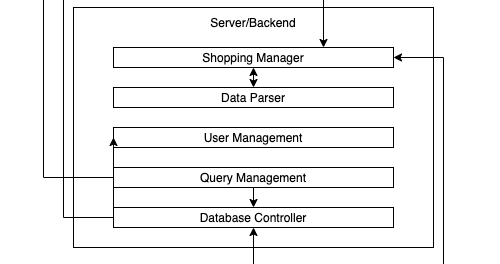
\includegraphics[width=0.60\textwidth]{images/backend}
 \caption{Back-End layer subsystem}
\end{figure}

\subsection{Shopping manager Subsystem}
The Shopping Manager Subsystem will deal with all the shopping related computation. It will get requests
directly from the shopping subsystem of the front-end. Then it will get the required shopping data
from the Data Controller layer.

\begin{figure}[h!]
	\centering
 	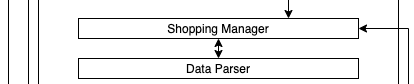
\includegraphics[width=0.60\textwidth]{images/ShoppingManager.png}
 \caption{Shopping manager Subsystem}
\end{figure}


\subsubsection{Subsystem Software Dependencies}
The subsystem will use the axios library to communicate with the Data Controller Layer. It will also use Google Maps library to display and calculate the optimum route to the user.

\subsubsection{Subsystem Programming Languages}
JavaScript (NodeJS)

\subsubsection{Subsystem Data Structures}
It will provide the front-end with the Prices and Availability of grocery items. Also the data required to display the optimum route on the front end.

\subsubsection{Subsystem Data Processing}
The shopping optimization algorithm will seek to find the best route given the users criteria.
To start with, define $\textbf{S} = \{S_1,S_2,...,S_n\}$ to be an ordered set of $n$ stores, to be visited, from $S_1$ to $S_n$ in order and define $S_0$ to be the starting location of the user.  Next, define $w_0$ and $w_1$ to be non-negative weights
defined by the user to give the importance of distance and item price, respectively.  Define $d(S_{i-1},S_i)$ to be the distance from $S_{i-1}$ to $S_i$ for all $i=1,2,...,n$.
Define $\lamda(S_i,h)$ to be the cost of item $h$ at store $S_i$.  Finally, define $\textbf{H}(S_i)$ to be the set of items the user is planning to buy at store $S_i$.  Thus, we are able to define our cost function as:
\begin{equation}
	COST(\textbf{S},\textbf{H}) := w_0\sum_{i=1}^n d(S_{i-1},S_i) + w_1\sum_{i=1}^n \sum_{h\in\textbf{H}(S_i)} \lambda(S_i,h)
\end{equation}
Hence, if $\textbf{A}$ represents the shopping list of the user, then it should follow that
\begin{equation}
	\textbf{A} =: \bigcup_{s\in\textbf{S}}\textbf{H}(s)
\end{equation}
provided all of the items on the shopping list are able to be found.
Thus, we can see that if $\textbf{S}$ is known, then $\textbf{H}$ follows by choosing the cheapest store for each item in $\textbf{A}$.  It also follows that $COST$ is monotonic with respect to the number of items in $\textbf{A}$.
Therefore, A-Star can be applied and shall be applied to this measure time, and should be of quadratic time complexity.
\subsection{User Management Subsystem}
The User Management Subsystem will handle all requests from the front-end related to the user of the
application and give back appropriate response. It will keep track of the currently logged in user.

\begin{figure}[h!]
	\centering
 	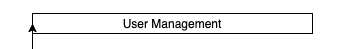
\includegraphics[width=0.60\textwidth]{images/UserManagement.png}
 \caption{User Management Subsystem}
\end{figure}


\subsubsection{Subsystem Software Dependencies}
This subsystem will Handle GoogleLogin authentication to make sure a user is logged in and connects their Google ID to the ID stored in the database. This subsystem will also use Axios library.

\subsubsection{Subsystem Programming Languages}
JavaScript (NodeJS) and SQL.

\subsubsection{Subsystem Data Structures}
This subsystem will create a data structure for the user's profile using the Google ID and send it to the front-end.

\subsubsection{Subsystem Data Processing}
It will take in the Google ID for the user, search for that stored Google ID in the database and pull all the data associated to that user.

\subsection{Query Management Subsystem}
The Query Management Subsystem will handle all requests from the front-end that needs a result from
a query on the database and give back the appropriate response.

\begin{figure}[h!]
	\centering
 	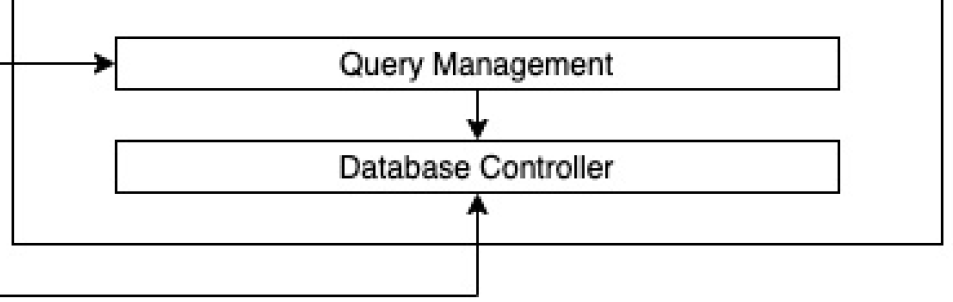
\includegraphics[width=0.60\textwidth]{images/Screenshot (61).png}
 \caption{Query Management Subsystem}
\end{figure}


\subsubsection{Subsystem Software Dependencies}
It will use the npm pg library to communicate with the PostgreSQL Database stored in Google Cloud Platform.

\subsubsection{Subsystem Programming Languages}
JavaScript (NodeJS) and SQL.

\subsubsection{Subsystem Data Structures}
This subsystem will be responsible for creating and managing all the queries to the database.

\subsubsection{Subsystem Data Processing}
Depending on the request, this layer will create a database query and send it to the Database Controller Layer.

\subsection{Database Controller Subsystem}
The database controller will handle all the communication of the application to the database. It will
give responses to the query management system with the required data extracted from the database.

% \begin{figure}[h!]
% 	\centering
%  	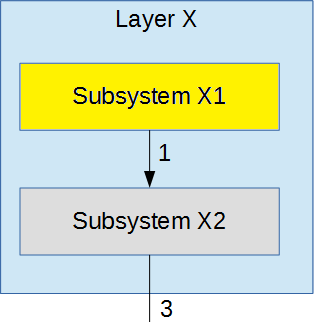
\includegraphics[width=0.60\textwidth]{images/subsystem}
%  \caption{Example subsystem description diagram}
% \end{figure}


\subsubsection{Subsystem Software Dependencies}
It will use the npm pg library to communicate with the PostgreSQL Database stored in Google Cloud Platform using Axios.

\subsubsection{Subsystem Programming Languages}
JavaScript (NodeJS) and SQL.

\subsubsection{Subsystem Data Structures}
This subsystem will take queries from the Query Management Layer and send those queries to the database.

\subsubsection{Subsystem Data Processing}
This subsystem will send the queries to the database and get the result and send it back to the Query Management Layer.